\section{Master}
% What responsibilities does M have?
% How is M structured?
% What models does M contain?
% What controllers should M contain, and what should be in these controllers?
% What views does M need?
% How should the web application of M look?

The structure of \deno{M}, as shown in Figure~\ref{fig:int_struct_m} is derived from the functionality of Master described in Section~\ref{sec:functionality_distribution}.
This figure shows three processes; Web, Database, and Daemon.
The Database process, \deno{DB} can be any database engine capable of handling transactions, therefore this will not be elaborated further.
The Web and Daemon processes will need further explanation, however. \\

\begin{figure}[htb]
    \centering
    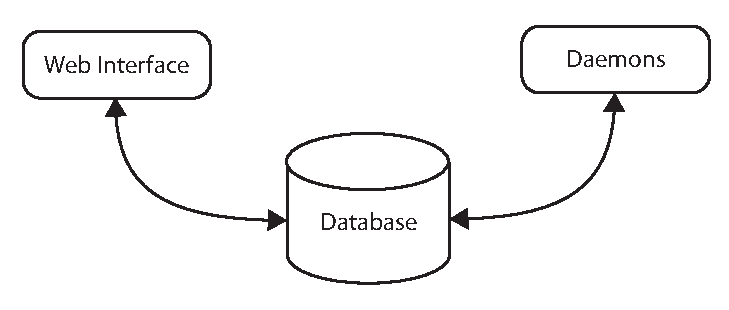
\includegraphics[width=0.7\textwidth]{gfx/master_internal_structure.pdf}
    \caption{Internal structure of Master}
    \label{fig:int_struct_m}
\end{figure}
\fxfatal{Skal der v�re noget der indikerer kommunimation til og fra daemon og web p� figuren.}

%%%%%  WEB   %%%%%
The web process, \deno{W} will be a web server using the Model-View-Controller (MVC) design pattern, see \citep{mvc}.
It consists of three layers, model, view, and controller.
There are several frameworks in different languages that support MVC, which will be considered in Section~\ref{sec:tools}. \\

The concept of MVC is decoupling the different layers to make it possible to develop them with some degree indepence.
As an example a method for fetching data in the model, can be changed without affecting the view, as long as its output format remains unchanged.
%Furthermore the developers can create several views for the same model.
%It also provides developers the opportunity to change how user input is handled in the controller without modifying the associated view.
Decoupling the layers forces the developer to keep the code separated, keeping code meant for the controller out of the view.
This separation means that the developer can isolate bugs to a specific layer, and can make debugging easier.

% The analysis of the problem domain provided the object model as described in Section~\ref{subsec:objects}.
% This model provides several models that are suitable for the MVC structure.

%MVC allows extending the functionality of each layer without touching the other layers and breaking working code.
%This does not mean that the developer can completely rewrite a layer without experiencing issues, but adding to a layer should leave the old code in a working state.
% Kodeopsplitning -> readability / debugging
% Analyse/Design -> Object Model gør at vi kan gøre alle vores tabeller til modeller
% Videreudvikling

In Section~\ref{subsec:objects} the object model is described.
The models of \deno{W}'s MVC are derived from this object model.
Each model will have a direct mapping to a table in \deno{DB}, and communication with the table in \deno{DB} must go through the model. \\

In order for a model to have a set of associated views it must have a controller.
In \projectname{} this includes models such as User, Drone, and Company, described in Section~\ref{subsec:objects}.
There will furthermore be controllers with no corresponding model, e.g. an access controller, which will handle login and logout.
Each controller in \projectname{} with a corresponding model, i.e. Affiliate Privilege, Company, Drone, Privilege, Role, and User, will have Create, Read, Update, and Delete (CRUD)\fxfatal{ref til CRUD} as default actions. All the controllers' actions are listed in Appendix~\ref{app:controller_actions} \\

%In the application there will be two ways of returning the information from a controller, either HTML \citep{what_is_html} or JSON \citep{what_is_json}.
%The JSON view will only contain the raw JSON, whereas the HTML will contain e.g. HTML tags, CSS, and Javascript.
%The JSON views will be used for asynchronously fetching data from the server, while the HTML views will be used for actions that require user input. \\

%%%%% DAEMON %%%%%
The daemon process, \deno{D}, has two tasks and will be a process running in the background of \deno{M}.
One of the purpose is to handle the session communication with \deno{S}.
Session communication refers to the session key required to communicate with a drone, as described in Section~\ref{sec:communication_network}.
\deno{D} will be written in the same language as \deno{W}. % to limit the amount of languages used.
\deno{D} will handle session communication with \deno{S} by continuously checking \deno{DB} for new session requests.
The session communication is handled through the \deno{DB}, to account for the asynchronous behaviour of the web\citep{stateless}.
This makes it possible to run multiple instances of \deno{D}, as they can use a shared queue in \deno{DB}.
If a session request is present in \deno{DB}, then \deno{D} will request a session from the associated \deno{S}.
If \deno{D} receives a valid session id from \deno{S}, it saves this in \deno{DB} and \deno{W} sends it to the user.
\deno{D} should handle session requests chronologically, thus if several requests are present in \deno{DB} then \deno{D} will not perform all requests simultaneously. 
The second purpose of \deno{D}, is to handle initialization messages from \deno{S}. 
\fxfatal{Rasmus was here. Skriv hvad initialization message er samt hvordan det mere teknisk fungere.}
\\


\deno{D} will handle the session requests as a First In, First Out (FIFO) queue.
However, since the response from \deno{S} can be delayed for an arbitrary amount of time, there is no guarantee that the first session request to be handled is also the first session to be entered in \deno{DB}.
\deno{S} will only return a valid session key, if it currently has no active sessions.
Therefore at most one person will have a valid session key for communicating with \deno{S} at any given time.
How this session key communication is handled can be seen in Figure~\ref{fig:sessionkey_communication_b}.

\begin{figure}[htb]
    \centering
    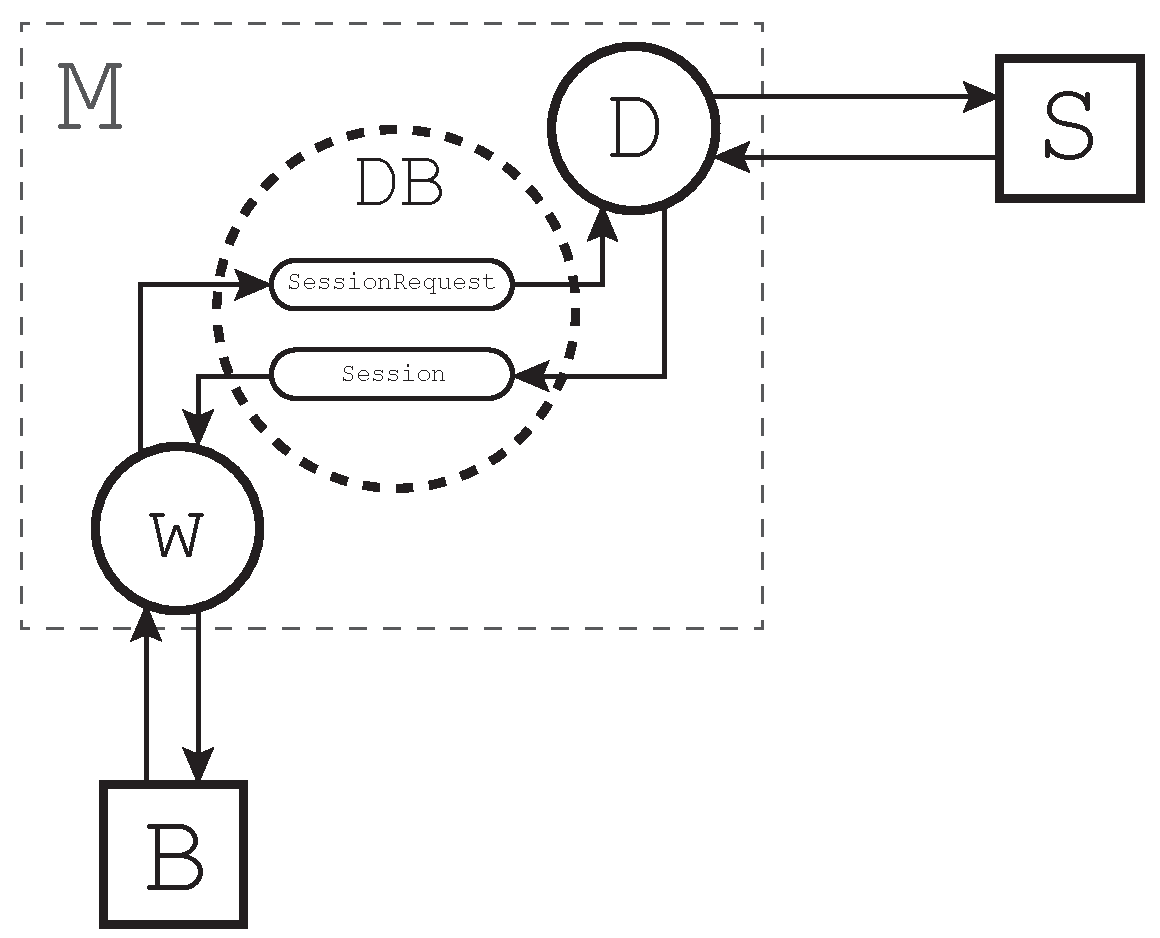
\includegraphics[width=0.85\textwidth]{gfx/sessionkey_communication_b.pdf}
    \caption{Session key communication.}
    \label{fig:sessionkey_communication_b}
\end{figure}

%%%%% DESIGN %%%%%
\subsection{Design language}
\fxfatal{Bjarke og Thomas tag stilling}
The design language, which is also known as design vocabulary, is the design guidelines for \projectname{}.
The objects here will have an important role in the systems user interface, and their design language is therefore described here.

\subsubsection{Color schema}
\begin{figure}[htb]
    \centering
    
\includegraphics[width=0.5\textwidth]{gfx/color_schema.pdf}
    \caption{Color schema of \projectname{}.}
    \label{fig:color_schema}
\end{figure}

The color schema seen in \figref{fig:color_schema} shows the colors that are being used in the applications design. \fixme{hvorfor har vi valgt de farver fremfor orange og lyserød?}

\subsubsection{Fonts}
The family of fonts will be: Arial, Helvetica.
These fonts have been selected because they are common both in Windows and Mac and therefore they are browser safe \cite{common_fonts}, meaning that the system will look the same no matter what operating system the user is using.

\subsubsection{Shapes}
All boxes that the user can interact with in the system, will be displayed with rounded corners.
This was done to make the interaction with the boxes as simple and straight forward as possible for the user.

\subsubsection{Layouts}
\begin{figure}[htb]
    \centering
    
\includegraphics[width=0.5\textwidth]{gfx/menu.pdf}
    \caption{The menu of the application, with the control menu point activated.}
    \label{fig:menu_design}
\end{figure}

In \figref{fig:menu_design} the menu of the application is seen.
In the figure, the bullet ``Control'' is active and therefore shown with a gray background color.
All other menus have a black background color and are separated with white spaces.

\begin{figure}[htb]
    \centering
    
\includegraphics[width=0.5\textwidth]{gfx/search.pdf}
    \caption{Search bar of the application}
    \label{fig:search_bar_design}
\end{figure}

In \figref{fig:search_bar_design} the search bar of the application is seen.
The ``search'' text will disappear when the bare is clicked, and if the user types anything this will be shown in the search bar instead.

\begin{figure}[htb]
    \centering
    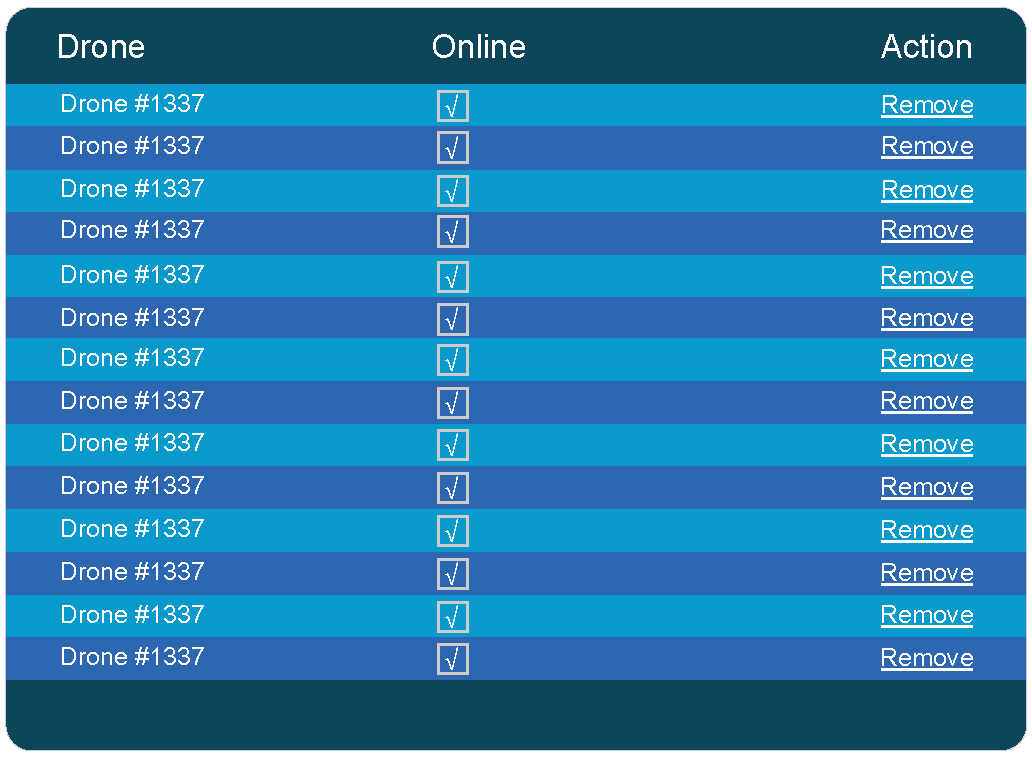
\includegraphics[width=0.7\textwidth]{gfx/table.pdf}
    \caption{Table design for the application.}
    \label{fig:table_design}
\end{figure}
In \figref{fig:table_design} the general design for tables of the application is seen.
Odd rows will be light blue and even rows will be blue.

\begin{figure}[htb]
    \centering
    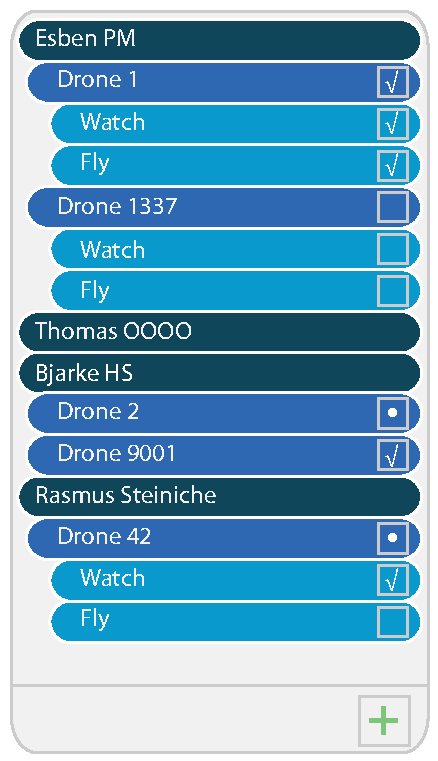
\includegraphics[width=0.5\textwidth]{gfx/list.pdf}
    \caption{List design for the application.}
    \label{fig:list_design}
\end{figure}
The list design shown in \figref{fig:list_design} is designed to show a tree-structured list.
This example shows the relationship between drones, privileges and users, where it is possible to activate different privileges on a given drone for a given user.
Each type of element (user, drone and privilege) as separate colors to make it easier to get an overview of the list. \\

Each privilege can have three different marks:

\begin{itemize}
    \item Not marked
    \item Dotted
    \item Ticked
\end{itemize}

If no privileges are marked, as seen with ``Drone 1337'', the user has no privileges to access this drone.
If a box is dotted, as seen with ``Drone 42'', the user s some privileges for this drone.
And finally, if a box is ticked, as seen with ``Drone 1'', the user has all privileges for this drone.

\begin{figure}[htb]
    \centering
    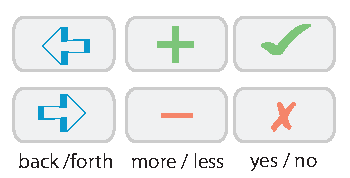
\includegraphics[width=0.5\textwidth]{gfx/button.pdf}
    \caption{Button design for the application.}
    \label{fig:button_design}
\end{figure}

The buttons used in \projectname{} has also gotten their own design to match the rest of the view.
There are six buttons:
Back, Forth, More, Less, Yes, \& No.
These will be used in the user interface where appropriate.
They do not carry any functionality, but are merely standard buttons with nicer looks.
